\documentclass{standalone}
\usepackage{tikz}
\usepackage{ctex,siunitx}
\usepackage{tkz-euclide}
\usepackage{amsmath}
\usetikzlibrary{patterns, calc}
\usetikzlibrary {decorations.pathmorphing, decorations.pathreplacing, decorations.shapes,}
\begin{document}
\small
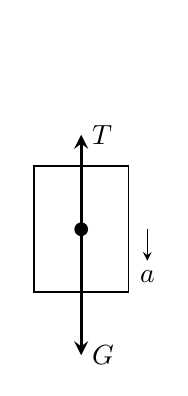
\begin{tikzpicture}[>=stealth,scale=0.8]
  \useasboundingbox(2.9,-1.2)rectangle(5,4.2);
  % \draw [semithick] (0,0) rectangle (1.5, 2);
  \draw [semithick] (3,0) rectangle (4.5, 2);
  % \draw [fill=black] (0.75,1)  circle [radius=.1];
  \draw [fill=black] (3.75,1)  circle [radius=.1];
  % \draw[<->, very thick] (.75, 4)node [right]{$T$}--(.75, -1)node [right]{$G$};
  \draw[<->, very thick] (3.75, 2.5)node [right]{$T$}--(3.75, -1)node [right]{$G$};
  % \draw [<-](1.8, 1)node [above]{$a$}--(1.8, .5);
  \draw [->](4.8, 1)--(4.8, .5)node [below]{$a$};
\end{tikzpicture}
\end{document}